\chapter{Bäume}

\begin{itemize}
  \item Verallg. von Listen: Element/Knoten kann mehrere Nachfolger haben
  \item Darstellung von Hierarchien
\end{itemize}

\paragraph{Ungerichteter Graph}
\index{Ungerichteter Graph}
$(V, E)$ mit einer Menge Knoten $V$ und Kanten $E \subseteq V \times V$

\paragraph{Baum}
\index{Baum}
Ungerichteter Graph mit

\begin{description}
  \item [Einfach] keine Schleife
        \mzInline{
          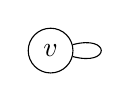
\begin{tikzpicture}[every loop/.style={}]
            \node [circle,draw] {$v$} edge[loop right] ();
          \end{tikzpicture}
        }
        oder Doppelkanten
        \mzInline{
          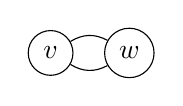
\begin{tikzpicture}
            \node (v) [circle,draw] {$v$};
            \node (w) at (1,0) [circle,draw] {$w$};
            \path (v) edge [bend left] (w);
            \path (w) edge [bend left] (v);
          \end{tikzpicture}
        }
        \index{Einfacher Graph}

  \item [Zusammenhängend]
        \index{Zusammenhängender Graph}
        Für jede zwei Knoten gibt es genau eine Folge von Kanten die sie verbindet

  \item [Azyklisch]
        \index{Azyklischer Graph}
        kein Zyklus (Cycle)
        \mzInline{
          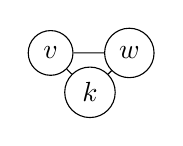
\begin{tikzpicture}
            \node (v) [circle,draw] {$v$};
            \node (w) at (1,0) [circle,draw] {$w$};
            \node (k) at (.5,-.5) [circle,draw] {$k$};

            \draw (v) -- (w) -- (k) -- (v);
          \end{tikzpicture}
        }
\end{description}

\paragraph{Wurzelbaum}
\index{Wurzelbaum}
Baum mit genau einem Knoten der Wurzel hei\ss t

\paragraph{Orientierter Wurzelbaum}
\index{Orientierter Wurzelbaum}
Alle Knoten sind Wurzel ihrer disjunkten Unterbäume und haben verschiedene Werte gleichen Typs. (Im Nachfolgenden einfach nur ,,Baum``)

% TODO: TikZ Grafik für Wurzelbaumterminologie

\paragraph{Darstellungsarten}

% TODO: TikZ Grafiken
\begin{description}
  \item[Graph]
    \mzInline{
      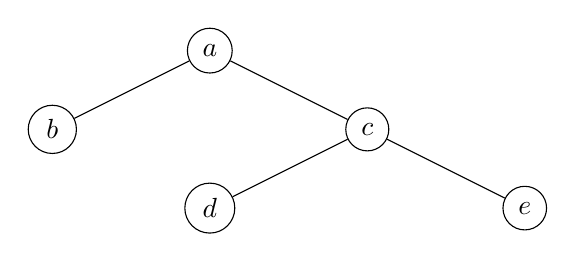
\begin{tikzpicture}[xscale=2]
        \node (b) at (0,0) [circle,draw] {$b$};
        \node (a) at (1,1) [circle,draw] {$a$};
        \node (c) at (2,0) [circle,draw] {$c$};
        \node (d) at (1,-1) [circle,draw] {$d$};
        \node (e) at (3,-1) [circle,draw] {$e$};

        \draw (b) -- (a) -- (c) -- (e);
        \draw (c) -- (d);
      \end{tikzpicture}
    }
    \mzInline{
      \begin{tikzpicture}[xscale=2]
        \node (b) at (0,0) [circle,draw] {$b$};
        \node (a) at (1,1) [circle,draw] {$a$};
        \node (c) at (2,0) [isosceles triangle,shape border rotate=90,draw] {$T_r$};

        \draw (b) -- (a) -- (c.apex);
      \end{tikzpicture}
    }
  \item[Array] $[a,b,c,\emptyset,\emptyset,d,e]$
    % \item[Verkettete Liste]
    % \item[Einrückung]
  \item[Menge] $\{\{a,b,c,d,e\},\{b\},\{c,d,e\},\{d\},\{e\}\}$
  \item[Klammer] $(a, (b), (c, (d), (e)))$
\end{description}

\paragraph{Grö\ss en}

\begin{description}
  \item[Ordnung] Max. Anzahl von Kindern jedes Knoten eines Baums
    \index{Baumordnung}

  \item[Tiefe] Anzahl Kanten zwischen einem Knoten und Wurzel
    \index{Knotentiefe}

  \item[Stufe] Alle Knoten gleicher Tiefe
    \index{Baumstufe}

  \item[Höhe] Max. Tiefe $+ 1$
    \index{Baumhöhe}
\end{description}

\paragraph{Eigenschaften}

\begin{description}
  \item[Geordnet] Kinder erfüllen Ordnung von links nach rechts
    \index{Geordneter Baum}

  \item[Vollständig]
    \index{Vollständiger Baum}
    Alle Blätter auf gleicher Stufe, jede Stufe hat max. Anzahl von Kindern
\end{description}

\section{Binärbäume}
\index{Binärbaum}

Geordneter, orientierter Wurzelbaum der Ordnung $2$.

\begin{description}
  \item[Strikt]
    \index{Strikter Binärbaum}
    Jeder Knoten hat $0$ oder $2$ Kinder (Kein Knoten hat genau $1$ Kind).

  \item[Vollständig]
    \index{Vollständiger Binärbaum}
    Jeder Knoten au\ss er der letzten Stufe hat genau $2$ Kinder.

  \item[Fast Vollständig]
    \index{Fast Vollständiger Binärbaum}
    Vollständig, außer Blätter können rechts fehlen.

  \item[Ausgeglichen]
    \index{Ausgeglichener Binärbaum}
    Vollständig, aber Blätter auf letzten $2$ Stufen
\end{description}

$2$ Binärbäume hei\ss en

\begin{description}
  \item[Ähnlich] selbe Struktur
    \index{Ähnliche Binärbäume}

  \item[Äquivalent] Ähnlich und selbe Knoten
    \index{Äquivalte Binärbäume}
\end{description}

\paragraph{Grö\ss en}

\begin{itemize}
  \item Für $i$ Stufen max. $2^i$ Knoten
  \item Für $n$ Knoten genau $n - 1$ Kanten
  \item Vollständiger B. mit $n$ Knoten hat Höhe von $\log_2 n + 1$
\end{itemize}